\begin{figure}[htbp]
	\centering
	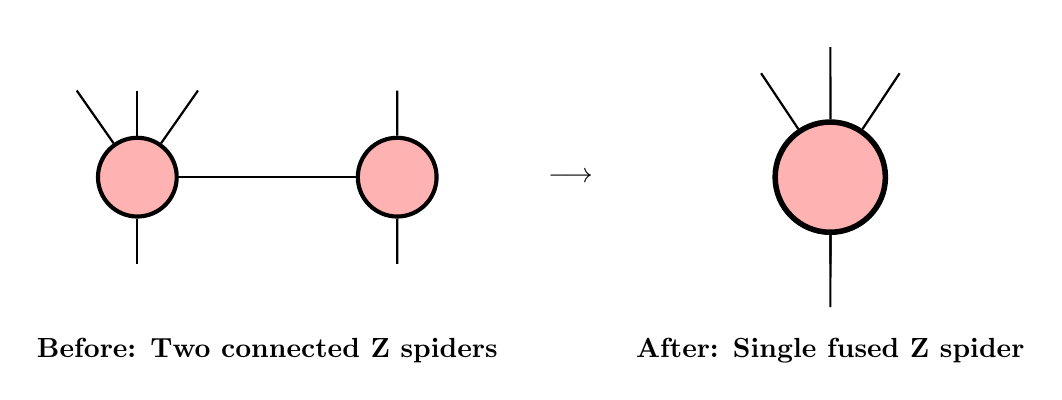
\begin{tikzpicture}[scale=1.1]
		\node[draw, circle, fill=red!30, minimum size=1cm, line width=1.5pt] (r1) at (0,0) {};
		\node[draw, circle, fill=red!30, minimum size=1cm, line width=1.5pt] (r2) at (3,0) {};
		\draw[thick] (r1) -- ++(0,1) node[above] {};
		\draw[thick] (r1) -- ++(-0.7,1);
		\draw[thick] (r1) -- ++(0.7,1);
		\draw[thick] (r1) -- ++(0,-1) node[below] {};
		\draw[thick] (r1) -- (r2);
		\draw[thick] (r2) -- ++(0,1) node[above] {};
		\draw[thick] (r2) -- ++(0,-1) node[below] {};

		\node at (1.5,-2) {\textbf{Before: Two connected Z spiders}};

		\node at (5,0) {$\longrightarrow$};

		\node[draw, circle, fill=red!30, minimum size=1.4cm, line width=2pt] (r3) at (8,0) {};
		\draw[thick] (r3) -- ++(0,1.5) node[above] {};
		\draw[thick] (r3) -- ++(-0.8,1.2);
		\draw[thick] (r3) -- ++(0.8,1.2);
		\draw[thick] (r3) -- ++(0,-1) node[below] {};
		\draw[thick] (r3) -- ++(0,-1.5) node[below] {};

		\node at (8,-2) {\textbf{After: Single fused Z spider}};

	\end{tikzpicture}
	\caption{The Spider Theorem in ZX calculus: two connected Z spiders fuse into a single Z spider. This fundamental rule enables simplification of ZX diagrams and reasoning about quantum operations. Spider Theorem (Fusion): When two spiders of the same color are connected, they fuse into a single spider. The total number of wires is preserved: $(m,n) \cup (n,p) = (m,p)$.}
	\label{fig:zx-spider-fusion}
\end{figure}
